\documentclass[sigconf,screen,nonacm]{acmart}

\settopmatter{printfolios=true}
\emergencystretch=1.5em

\begin{document}

\title{Workload-Specific Physical Memory Efficiency and Bounded Page Reclamation for Dedicated Edge Computer Vision Inference}

\author{Erdeni Khatunov}
\affiliation{%
  \department{Student ID: 126033990029 \textbar{} Group: GE6001-03300-M03}
  \institution{Shanghai Jiao Tong University}
  \city{Shanghai}
  \country{China}
}
\email{r_sp_alloc}

\begin{abstract}
High DRAM costs make physical memory capacity a primary constraint for dedicated edge computer vision deployments such as factory inspection and traffic analytics. Yet conventional user-space allocators and inference runtime arenas are built with defensive caching, guardrails, and retention policies tailored to general-purpose multi-tenant software, causing dedicated inference services to pin substantial unused physical memory across idle intervals. This report presents our research on workload-specific memory efficiency in the \texttt{r\_sp\_alloc} project, evaluated on fixed-shape FP32 YOLO26n inference under ONNX Runtime. Grounded in recent analyses of user-kernel page-granularity mismatch (Fistanto et al., PLOS '26) and custom allocator trade-offs (van Kempen and Berger, ISMM '26), we investigate \texttt{PageReuseResource}, an out-of-band coalescing allocator integrated with bounded pause-time page reclamation (\texttt{purge\_to\_budget}). Across two recent development milestones, full pause purging (\texttt{c9828c5}) cut idle private RAM by 71.1\% but degraded p99 tail latency by 11.1\% due to resume page faults. Introducing a 24~MiB resident free-page budget (\texttt{1fd7ede}) eliminated that regression, achieving a 50.8\%--50.9\% idle private RAM reduction, 44.0\%--44.3\% estimated private byte-seconds savings, under 1\% active FPS loss, and a median burst p99 ratio of 1.0108 with zero FP32 numerical error.
\end{abstract}

\keywords{Edge Computer Vision, Physical Memory Efficiency, Page Reclamation, Custom Memory Allocation, ONNX Runtime}

\maketitle

\section{Introduction}
Edge computer vision appliances---including automated optical defect inspection lines, warehouse robotics, and multi-camera traffic gateways---execute continuous deep-learning inference on compact Linux nodes where DRAM dominates hardware cost and caps workload density. When physical memory is scarce, operators must either under-provision concurrent video streams or accept costly hardware upgrades, swapping stalls, or accuracy loss from reduced input resolution and quantization.

Despite predictable, repetitive tensor allocation patterns, dedicated edge inference processes typically run atop general-purpose memory stacks designed for unpredictable multi-user programs. Allocators such as GNU \texttt{glibc malloc}, \texttt{jemalloc}~\cite{evans2006jemalloc}, \texttt{TCMalloc}~\cite{ghemawat2005tcmalloc}, and \texttt{mimalloc}~\cite{leijen2019mimalloc}, alongside inference runtime arenas such as ONNX Runtime's Best-Fit with Coalescing (BFC) CPU allocator, rely on per-thread caches, geometric chunk growth, and deferred reclamation to minimize lock contention and kernel system calls. In dedicated production deployments, however, those safeguards retain freed virtual buffers indefinitely after inference frames finish, keeping 4~KiB physical pages pinned in RAM even while cameras wait between triggered bursts.

Two recent 2026 systems studies sharpen our understanding of this waste. Fistanto, Tempel, and Dietrich~\cite{fistanto2026lostbytes} formalize the granularity mismatch between user-space allocator blocks and Linux 4~KiB pages, partitioning freed regions into \textit{sub-page}, \textit{head}, \textit{tail}, and reclaimable whole-page \textit{body} holes. Merely coalescing freed blocks in user space leaves physical DRAM untouched unless empty page interiors are explicitly returned to the kernel via \texttt{madvise(..., MADV\_DONTNEED)}; conversely, simply over-aligning every small allocation to 4~KiB proves neither low internal waste nor effective physical reclamation. Moreover, their 75\% illustrative example concerns accumulated hole size rather than a universal reduction in total application resident set size (RSS), since static weights and shared libraries still remain resident. Complementing this view, van Kempen and Berger~\cite{vankempen2026reconsidering} revisit custom versus general-purpose allocation~\cite{berger2002reconsidering}, identifying deferred region deallocation as a direct source of memory inflation (Section~2.2.2) and introducing adversarial occupancy schedules (\textsc{Adv1}, \textsc{Adv3}, and \textsc{Adv10} at 0.33, 0.66, and 0.80) to expose fragmentation behavior when allocations interleave across time. Importantly, their evaluation focuses on single-threaded execution and emphasizes that cache-locality improvements alone do not establish lower physical memory consumption.

Building on these foundations, this report documents our ongoing work in \texttt{r\_sp\_alloc} under Graduate English assignment reporting guidelines. Specifically, we present: (1) an out-of-band coalescing allocator (\texttt{PageReuseResource}) that isolates metadata from purgeable mappings and verifies physical residency conservation via \texttt{mincore()}; (2) controlled repeatability and burst-mode evaluations across the last two commits (\texttt{c9828c5} and \texttt{1fd7ede}); and (3) a bounded pause-time retention mechanism (\texttt{purge\_to\_budget}) that halves idle private RAM without triggering the tail-latency regressions of full pause purging.

\section{Problem Statement and Acceptance Criteria}
Smart-camera edge pipelines commonly alternate between active inference bursts and quiescent pauses during which the ONNX Runtime session, model weights, and caller-retained output tensors must remain resident for rapid resumption. Under this bursty duty cycle, existing memory management strategies fall into three unsatisfactory regimes:

\begin{itemize}
  \item \textbf{Unbounded Arena Retention (Default BFC):} Retaining every allocated chunk eliminates recurring minor page faults (2 faults across 120--1,000 frames) and minimizes latency jitter, but holds roughly 119~MiB of idle private RAM per single-camera process and over 390~MiB across four live camera sessions, yielding allocator-local idle payload utilization as low as 20.8\%.
  \item \textbf{Per-Frame Trimming (\texttt{direct\_trim} / \texttt{direct\_every}):} Bypassing the CPU arena and trimming \texttt{glibc} pages on every frame reduces idle private RAM to $\sim$34.2~MiB, but forces continuous page zero-filling and kernel fault handling---incurring over 1.09~million minor page faults per 120 frames and dropping throughput from 6.33--6.46~FPS to 5.63--5.83~FPS.
  \item \textbf{Full Pause-Boundary Purging (\texttt{pool\_idle}, 0~MiB budget):} Retaining buffers during bursts and purging all empty page bodies at pauses limits throughput loss to $\sim$1.5\%, but leaves zero warm pages for the first frame after sleep, degrading p99 tail latency by 11.1\%.
\end{itemize}

To avoid misleading allocator comparisons, we enforced four pre-registered acceptance gates prior to running experiments: (1) \textbf{bit-exact numerical equivalence} (\texttt{max\_abs\_error == 0}) across complete FP32 output tensors and caller-retained outputs held across subsequent frames; (2) \textbf{live-session physical measurement} using Linux \texttt{mincore()} and \texttt{/proc/self/smaps\_rollup} rather than virtual reservations or teardown-only snapshots; (3) \textbf{$\ge$50\% idle private RAM reduction} versus BFC alongside lower time-integrated private byte-seconds; and (4) \textbf{bounded latency and throughput cost}, retaining $\ge$97\% continuous BFC FPS ($\le$3\% loss) and keeping median burst p99 latency within an assumed 5\% research materiality margin (ratio $\le 1.05$).

\section{System Architecture and Methodology}

\subsection{Workload and Bare-Metal Testbed}
All utilization experiments execute a fixed-shape $640 \times 640$ FP32 \textbf{YOLO26n} detector~\cite{jocher2026yolo26} via ONNX Runtime's CPU Execution Provider with full graph optimizations and memory-pattern planning enabled (single-thread intra-op and inter-op per session). Measurements run on a bare-metal CloudLab node (Intel Xeon D-1548 at 2.00~GHz, Broadwell-DE, 8~cores / 16~threads, 12~MiB L3, 64~GiB DRAM) running Ubuntu Linux (kernel \texttt{6.8.0-147-generic}, \texttt{g++ 13.3.0}), 4~KiB pages, Transparent Huge Pages disabled (\texttt{[never]}), and the \texttt{performance} CPU governor. Single-stream jobs are pinned to CPU core~2 using \texttt{sched\_\allowbreak setaffinity}, whereas four-camera runs pin workers across cores~0--3. Every accepted run checks complete output tensors against saved BFC FP32 references over eight deterministic inputs.

\begin{figure*}[t]
  \centering
  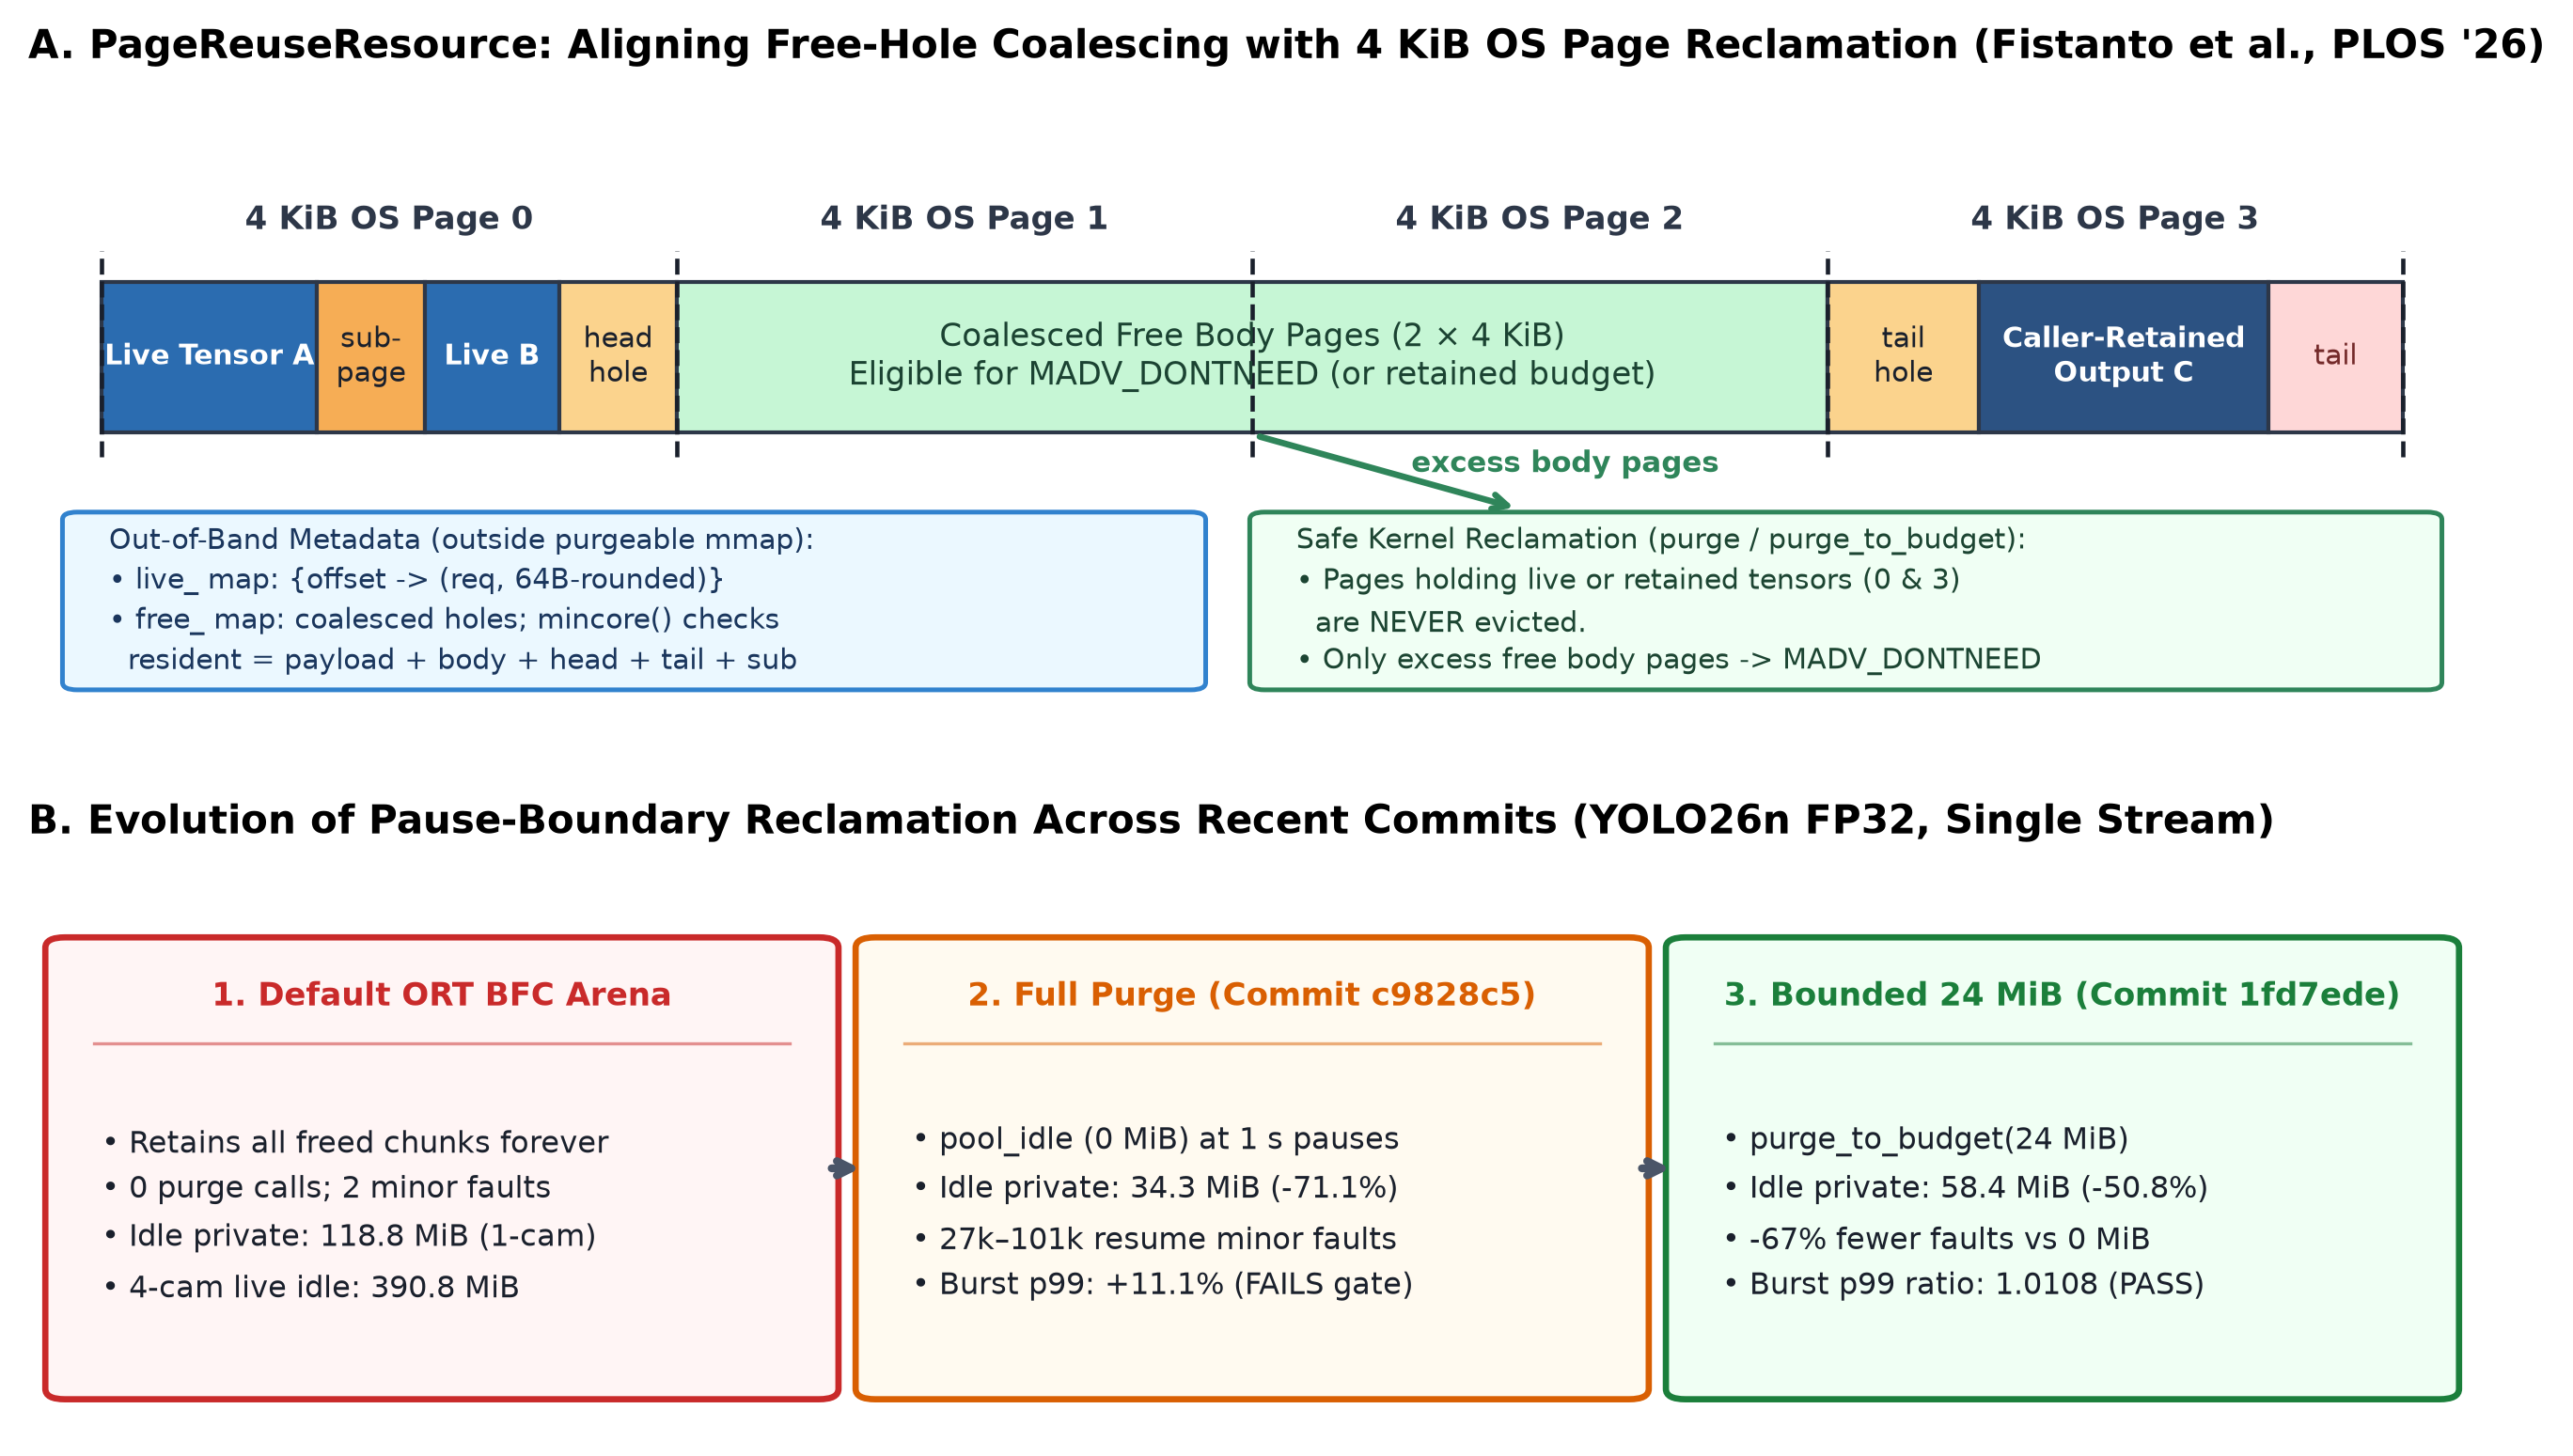
\includegraphics[width=\textwidth]{figures/fig1_architecture_holes.png}
  \caption{System design and recent commit progression in \texttt{r\_sp\_alloc}. (A) Mapping between user-space tensor allocations, caller-retained outputs, and 4~KiB OS pages in \texttt{PageReuseResource}, applying Fistanto et al.'s~\cite{fistanto2026lostbytes} hole taxonomy with out-of-band metadata isolation. (B) Progression from unbounded BFC retention to full pause purging (\texttt{c9828c5}) and bounded retention (\texttt{1fd7ede}).}
  \label{fig:arch}
\end{figure*}

\subsection{PageReuseResource Design}
To control the boundary between user-space chunk reuse and kernel page residency, we built \texttt{PageReuseResource} (\texttt{page\_\allowbreak reuse\_\allowbreak resource.hpp}) and registered it as a custom \texttt{OrtAllocator} via \texttt{ObservedAllocator} with ONNX Runtime's CPU arena disabled (\texttt{DisableCpuMemArena}) and environment-level allocator routing enabled. Each pool reserves 256~MiB of anonymous virtual address space via \texttt{mmap} (tracked separately from physical consumption) and rounds every request up to 64~bytes to match ONNX Runtime's tensor alignment without padding every small buffer to 4~KiB. Critically, all allocator bookkeeping structures---a \texttt{live\_} map recording requested and 64-byte-rounded sizes and a \texttt{free\_} map tracking free offset intervals---reside \textit{outside} the purgeable \texttt{mmap} mapping so metadata pages are never evicted and foreign-pointer or double-free errors are caught immediately.

When ONNX Runtime frees a tensor, \texttt{PageReuseResource} performs eager two-sided coalescing with adjacent left and right intervals in \texttt{free\_} and services subsequent allocations via best-fit search across coalesced intervals. At reclamation checkpoints, \texttt{discard(start, length)} rounds the interval start \textit{up} to the next 4~KiB page boundary and the interval end \textit{down} to the preceding page boundary (Figure~\ref{fig:arch}A): partial pages holding live or caller-retained tensors (\textit{sub-page}, \textit{head}, and \textit{tail} holes) remain untouched, while wholly free \textit{body} pages between those aligned bounds are discarded via \texttt{madvise(..., MADV\_DONTNEED)}. To guard against accounting drift, the built-in \texttt{sample()} routine queries Linux \texttt{mincore()} across every page in the mapping and asserts exact byte conservation:
\[
  \mathrm{resident} = \mathrm{payload} + \mathrm{body} + \mathrm{head} + \mathrm{tail} + \mathrm{sub}.
\]

\subsection{Progress Across Recent Commits}
Our experimental workflow progressed through two disciplined stages recorded in the last two commits (Figure~\ref{fig:arch}B):
\begin{enumerate}
  \item \textbf{Repeatability Audit and Pause Purging (\texttt{c9828c5}, Nov~9, 2026):} A 46-run randomized rerun (\texttt{recheck\_\allowbreak validation.py}) first verified prior baseline utilization measurements. Next, \texttt{activity\_\allowbreak bench.cpp} introduced bursty single-stream evaluation (10~warmup frames followed by 120~measured frames divided by scheduled 1~s pauses, holding one caller-retained output vector alive across an 11-frame window via \texttt{i \% 11}), isolating active inference and deallocation timings from reference verification, \texttt{/proc} sampling, and pause reclamation cost. Under \texttt{pool\_\allowbreak idle}, all free page bodies were purged upon entering each pause (0~MiB budget).
  \item \textbf{Bounded Free-Page Retention (\texttt{1fd7ede}, Nov~19, 2026):} To cushion cold-page faults on burst resumption, we added \texttt{purge\_\allowbreak to\_\allowbreak budget(\allowbreak size\_t budget)}. At pause entry, the routine scans \texttt{mincore()} residency across coalesced free intervals, skips over up to \texttt{budget / 4096} already-resident wholly free pages to keep a warm working-set reserve in RAM, and invokes \texttt{MADV\_\allowbreak DONTNEED} only on excess free pages beyond that budget. Following a pre-registered protocol (\texttt{PROTOCOL.md}), candidate budgets of 0, 8, 16, and 24~MiB were screened once in shuffled order against BFC; the script automatically froze the lowest-p99 candidate satisfying the $\le$50\% idle RAM threshold (24~MiB) prior to running five alternating-order fresh-process confirmation pairs (continuous and 10-frame bursts), a 1,000-frame endurance run (100~pauses), and a five-block shuffled 30-frame burst sensitivity check.
\end{enumerate}

\section{Experimental Evaluation}

\subsection{Baseline Utilization and Repeatability}
Table~\ref{tab:baseline} anchors our recent activity-aware experiments against single-stream (60~measured + 10~warmup frames) and four-camera (30~measured + 5~warmup frames per stream) baselines across both the initial utilization suite (\texttt{20dc7b8}) and the 46-run randomized recheck (\texttt{c9828c5}). Disabling ORT's CPU arena with \texttt{glibc} trimming (\texttt{direct\_\allowbreak trim}) cut single-stream median active peak RSS by 40.27\% versus default BFC (73.39 vs.\ 122.86~MiB; recheck 73.27 vs.\ 122.77~MiB) and reduced live idle private RAM from 119.06 to 34.20~MiB. Across conventional system allocators without explicit page-return hooks, \texttt{direct\_\allowbreak jemalloc} and \texttt{direct\_\allowbreak mimalloc} lowered idle private RAM to 35.84~MiB and 38.87~MiB but still reached higher active peak RSS (95.20~MiB and 78.14~MiB) than \texttt{direct\_\allowbreak trim}. Our custom \texttt{pool\_\allowbreak eager\_\allowbreak trim} matched this steady active footprint closely (73.74~MiB, +0.48\% over \texttt{direct\_\allowbreak trim}; recheck 73.62~MiB)---meaning we explicitly make no claim of custom-allocator dominance over tuned \texttt{glibc} trimming in single-stream peak RSS---while lowering startup peak RSS (73.50 vs.\ 78.99~MiB) and achieving lower four-camera live idle private memory (88.05 vs.\ 90.50~MiB, compared with 390.80~MiB under \texttt{bfc\_\allowbreak trim}). In a 1,000-frame continuous endurance pass, \texttt{direct\_\allowbreak trim} and \texttt{pool\_\allowbreak eager\_\allowbreak trim} maintained bounded footprints (73.34 and 73.82~MiB active peak; 34.20 and 34.44~MiB idle private) with zero output error.

Within the custom pool mapping itself, \texttt{mincore()} byte accounting confirmed why unpurged retention wastes physical RAM. When free ranges were retained without advising the kernel (\texttt{pool\_\allowbreak retain\_\allowbreak trim}), 44.96~MiB remained resident in the pool for 9.35~MiB of live ORT requests, trapping 35.61~MiB in completely free \textit{body} pages (37,344,184~B of resident waste) and yielding 20.7955\% allocator-local payload utilization. Adding eager coalescing and whole-page purging (\texttt{pool\_\allowbreak eager\_\allowbreak trim} and \texttt{pool\_\allowbreak boundary\_\allowbreak trim}) eliminated all free-body pages (0~B), leaving only 952~B of alignment/sub-page waste across 9.35~MiB of live requests and raising allocator-local idle payload utilization to 99.9903\%. This ratio strictly characterizes pool-owned mappings rather than whole-process DRAM. In addition, single-run synthetic stress checks adapted from ISMM '26 (\textsc{Adv1}/\textsc{Adv3}/\textsc{Adv10} at 0.33/0.66/0.80 occupancy using an empirical size histogram and 20,000 peak-object proxy) kept four-camera idle private RAM at 88.76--106.89~MiB under \texttt{pool\_\allowbreak eager\_\allowbreak trim} versus 390.68--409.09~MiB under \texttt{bfc\_\allowbreak trim}.

\begin{table*}[t]
  \centering
  \caption{Live-session physical RAM footprint across allocators (median [min, max] in MiB, five fresh processes per policy). Sources: \texttt{UTILIZATION\_REPORT.md} (\texttt{20dc7b8}) and randomized \texttt{RECHECK\_REPORT.md} (\texttt{c9828c5}). All outputs matched FP32 references bit-exactly.}
  \label{tab:baseline}
  \small
  \begin{tabular}{@{}lrrrrr@{}}
    \toprule
    \textbf{Regime / Policy} & \textbf{Startup Peak RSS} & \textbf{Active Peak RSS} & \textbf{Live Idle Private} & \textbf{Recheck Active Peak} & \textbf{Recheck Idle Private} \\
    \midrule
    Single: \texttt{bfc} (default)    & 122.86 [122.66, 123.16] & 122.86 [122.66, 123.16] & 119.06 [118.97, 119.36] & 122.77 [122.67, 123.16] & 118.96 \\
    Single: \texttt{bfc\_trim}        & 113.83 [113.44, 114.05] & 113.83 [113.44, 114.05] & 110.03 [109.64, 110.35] & 113.45 [113.42, 113.84] & 109.65 \\
    Single: \texttt{direct\_jemalloc} & 96.14 [95.15, 99.59]    & 95.20 [88.60, 99.41]    & 35.84 [35.79, 35.86]    & ---                     & ---    \\
    Single: \texttt{direct\_mimalloc} & 91.07 [86.52, 107.09]   & 78.14 [77.93, 78.50]    & 38.87 [38.86, 39.24]    & ---                     & ---    \\
    Single: \texttt{direct\_trim}     & 78.99 [78.86, 79.04]    & 73.39 [73.13, 73.40]    & 34.20 [34.18, 34.21]    & 73.27 [73.12, 73.39]    & 34.20  \\
    Single: \texttt{pool\_eager\_trim}& \textbf{73.50} [73.38, 73.69] & 73.74 [73.49, 73.80] & 34.43 [34.41, 34.43]    & 73.62 [73.61, 73.74]    & 34.42  \\
    \midrule
    4-Cam: \texttt{bfc\_trim}         & ---                     & 394.66 [393.50, 395.18] & 390.80 [389.65, 391.31] & 394.04 [393.67, 394.89] & 390.16 \\
    4-Cam: \texttt{direct\_trim}      & ---                     & 236.51 [236.45, 236.62] & 90.50 [90.39, 90.54]    & 236.27 [228.76, 236.59] & 90.42  \\
    4-Cam: \texttt{pool\_eager\_trim} & ---                     & \textbf{234.09} [233.81, 234.15] & \textbf{88.05} [88.02, 88.07] & \textbf{233.85} [222.69, 234.04] & \textbf{87.95} \\
    \bottomrule
  \end{tabular}
\end{table*}

\subsection{Full Pause-Boundary Purging (\texttt{c9828c5})}
Initial screening in \texttt{c9828c5} (120 frames, 30-frame bursts, 1~s pauses) contrasted default \texttt{bfc} against \texttt{direct\_\allowbreak every} (per-frame \texttt{malloc\_\allowbreak trim}), \texttt{direct\_\allowbreak idle} (pause-only \texttt{malloc\_\allowbreak trim}), and \texttt{pool\_\allowbreak idle}. Both \texttt{direct} policies triggered over 1.09~million minor page faults and dropped active throughput to 5.633--5.635~FPS (with \texttt{direct\_\allowbreak idle} peaking at 342.006~ms p99), whereas \texttt{pool\_\allowbreak idle} held 6.268~FPS with 27,368 faults and 290.357~ms p99. Advancing \texttt{pool\_\allowbreak idle} and \texttt{bfc} to five fresh burst repetitions confirmed the promise and residual gap of unbudgeted pause purging: \texttt{pool\_\allowbreak idle} slashed median idle private RAM by 71.1\% (34.344 vs.\ 118.703~MiB) and cut estimated private byte-seconds by 43.6\% ($1.597 \times 10^9$ vs.\ $2.830 \times 10^9$~B$\cdot$s), while keeping active throughput within 1.5\% (6.308 vs.\ 6.405~FPS). However, purging all free pages still forced $\sim$27,368 minor faults across the four pauses, driving median p99 latency from 268.918~ms up to 298.870~ms (+11.1\%). Because this exceeded the 5\% p99 gate, \texttt{c9828c5} explicitly documented that latency acceptance was not yet met.

\subsection{Bounded Retention Evaluation (\texttt{1fd7ede})}
Commit \texttt{1fd7ede} addressed that fault spike through bounded retention. During the 10-frame burst screening sweep (120~frames, twelve 1~s pauses, Figure~\ref{fig:screening}), expanding the free-page budget from 0 to 8, 16, and 24~MiB cut minor page faults by 67.3\% (from 100,517 down to 77,965, 55,427, and 32,918), reduced total pause reclamation time from 27.87 to 11.75~ms, and brought p99 latency down from 311.81 to 306.88~ms. Because 24~MiB yielded the lowest p99 latency while staying below half of BFC's idle private memory (58.34 vs.\ 118.79~MiB), it was frozen for paired confirmation.

\begin{figure*}[t]
  \centering
  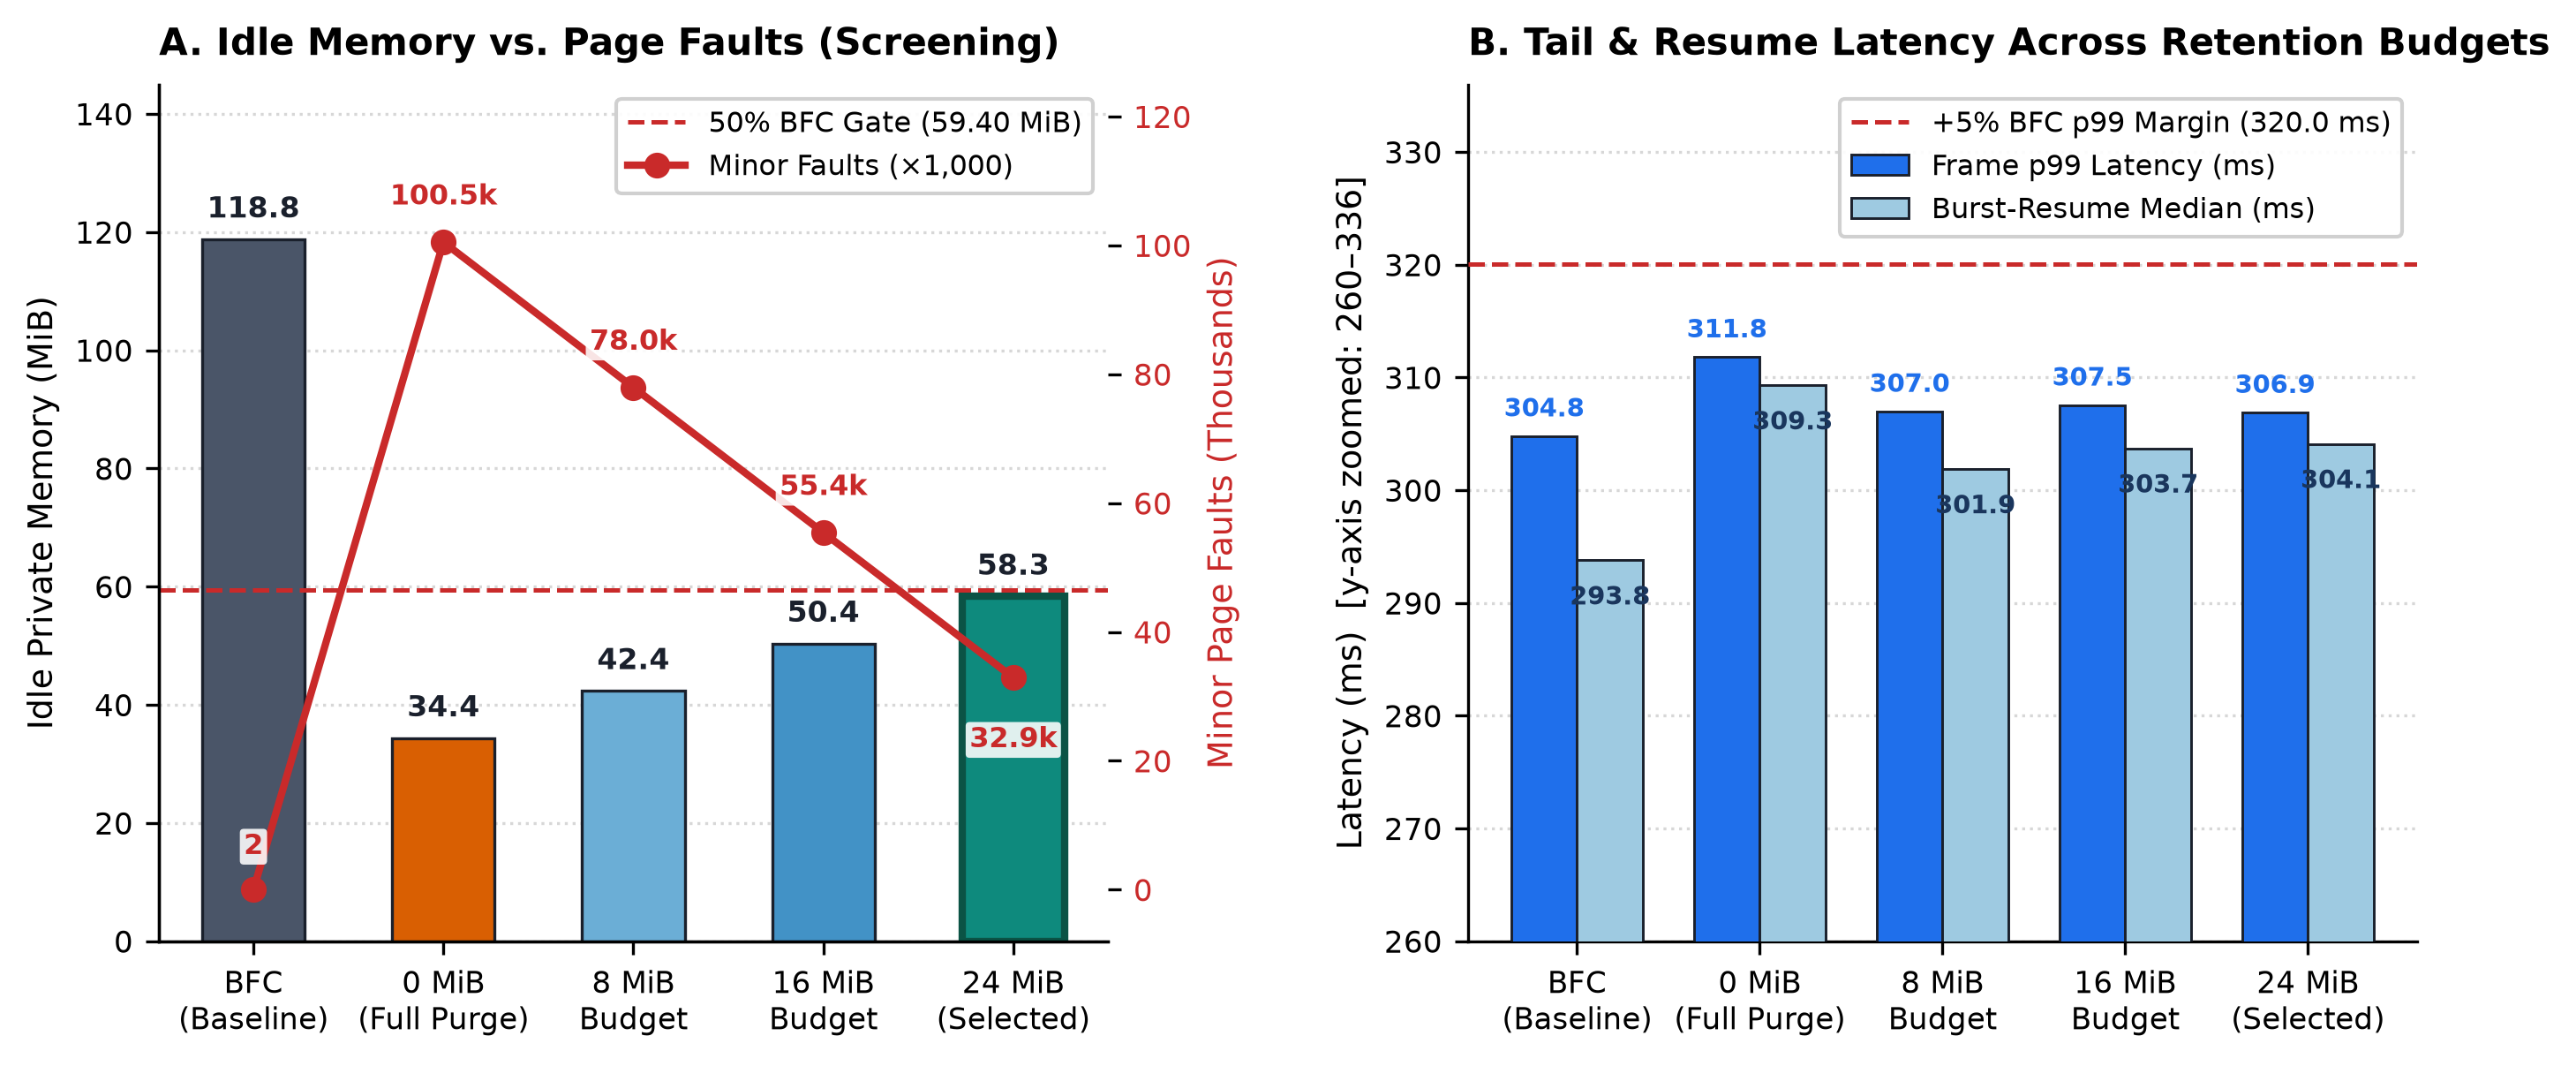
\includegraphics[width=\textwidth]{figures/fig2_bounded_screening.png}
  \caption{Pre-registered screening across BFC and \texttt{pool\_idle} retention budgets of 0, 8, 16, and 24~MiB (120~frames, 10-frame bursts, twelve 1~s pauses). A 24~MiB budget cuts minor page faults by 67.3\% relative to full purging while keeping idle private RAM below the 50\% BFC cutoff (59.40~MiB).}
  \label{fig:screening}
\end{figure*}

Table~\ref{tab:bounded} and Figure~\ref{fig:bounded} summarize the confirmed five-pair ratios, the 30-frame shuffled sensitivity check, and the 1,000-frame endurance run. Under confirmed 10-frame bursts, 24~MiB bounded retention delivered a median candidate/BFC idle private RAM ratio of 0.4916 ($-$50.8\%) and estimated private byte-seconds ratio of 0.5604 ($-$44.0\%), while holding continuous FPS at 0.9977, burst FPS at 0.9947, burst resume median latency at 1.0321, and burst p99 latency at 1.0108---passing every pre-registered median gate. Crucially, compared with the continuous regime where pauses do not occur and memory stays warm, bounded retention isolates physical reclamation strictly to idle gaps while preserving active working-set pages across frames. In the 30-frame sensitivity check, median p99 ratio improved slightly from 1.0500 (0~MiB) to 1.0474 (24~MiB) at a 0.4912 idle private RAM ratio, confirming the trade-off between full purging (maximum idle savings at borderline tail latency) and bounded buffering (50.9\% idle reduction with smoother burst resumption). Over 1,000 endurance frames (100 scheduled pauses), 24~MiB retention sustained 5.751 versus 5.796 active FPS ($-$0.8\%) and 290.87 versus 277.87~ms p99 (+4.7\%) while cutting idle private RAM from 118.79 to 58.37~MiB ($-$50.9\%) and total byte-seconds from 33.95 to 18.91~GB$\cdot$s ($-$44.3\%), incurring only 95.47~ms total pause reclamation overhead across all 100 pauses ($<$1~ms per pause) and zero output error.

\begin{table*}[t]
  \centering
  \caption{Confirmed paired ratios (24~MiB Bounded / BFC, $n=5$ pairs per regime), 30-frame sensitivity checks, and 1,000-frame endurance metrics (commit \texttt{1fd7ede}). All outputs passed exact FP32 verification (\texttt{max\_abs\_error = 0}).}
  \label{tab:bounded}
  \small
  \setlength{\tabcolsep}{4.5pt}
  \begin{tabular}{@{}llrrrl@{}}
    \toprule
    \textbf{Regime} & \textbf{Metric} & \textbf{Median (or 24~MiB)} & \textbf{Min (or BFC)} & \textbf{Max (or $\Delta$)} & \textbf{Status} \\
    \midrule
    Continuous (no pause) & Active FPS ratio         & 0.9977 & 0.9794 & 1.0107 & PASS ($\ge 0.97$) \\
    Continuous (no pause) & p99 latency ratio        & 1.0182 & 0.9895 & 1.2737 & Diagnostic (high max) \\
    Burst (10f, 1~s pause)& Active FPS ratio         & 0.9947 & 0.9892 & 1.0068 & Diagnostic \\
    Burst (10f, 1~s pause)& p99 latency ratio        & \textbf{1.0108} & 0.9359 & 1.0362 & PASS ($\le 1.05$) \\
    Burst (10f, 1~s pause)& Idle private RAM ratio   & \textbf{0.4916} & 0.4896 & 0.4918 & PASS ($\le 0.50$) \\
    Burst (10f, 1~s pause)& Est.\ private B$\cdot$s ratio & \textbf{0.5604} & 0.5537 & 0.5626 & PASS ($< 1.00$) \\
    Burst (10f, 1~s pause)& Resume median ratio      & 1.0321 & 1.0167 & 1.0334 & Diagnostic (+3.2\%) \\
    \midrule
    Sensitivity (30f, 0~MiB)  & p99 / Idle private ratio & 1.0500 / 0.2891 & 0.9945 / 0.2884 & 1.1473 / 0.2897 & Borderline p99 \\
    Sensitivity (30f, 24~MiB) & p99 / Idle private ratio & 1.0474 / 0.4912 & 0.9184 / 0.4899 & 1.1541 / 0.4918 & Median PASS (dispersed) \\
    \midrule
    Endurance (1,000f, 100p) & Idle (MiB) / p99 (ms) / FPS & 58.37 / 290.87 / 5.751 & 118.79 / 277.87 / 5.796 & $-$50.9\% / +4.7\% / $-$0.8\% & 296,226 vs.\ 2 faults \\
    \bottomrule
  \end{tabular}
\end{table*}

\begin{figure*}[t]
  \centering
  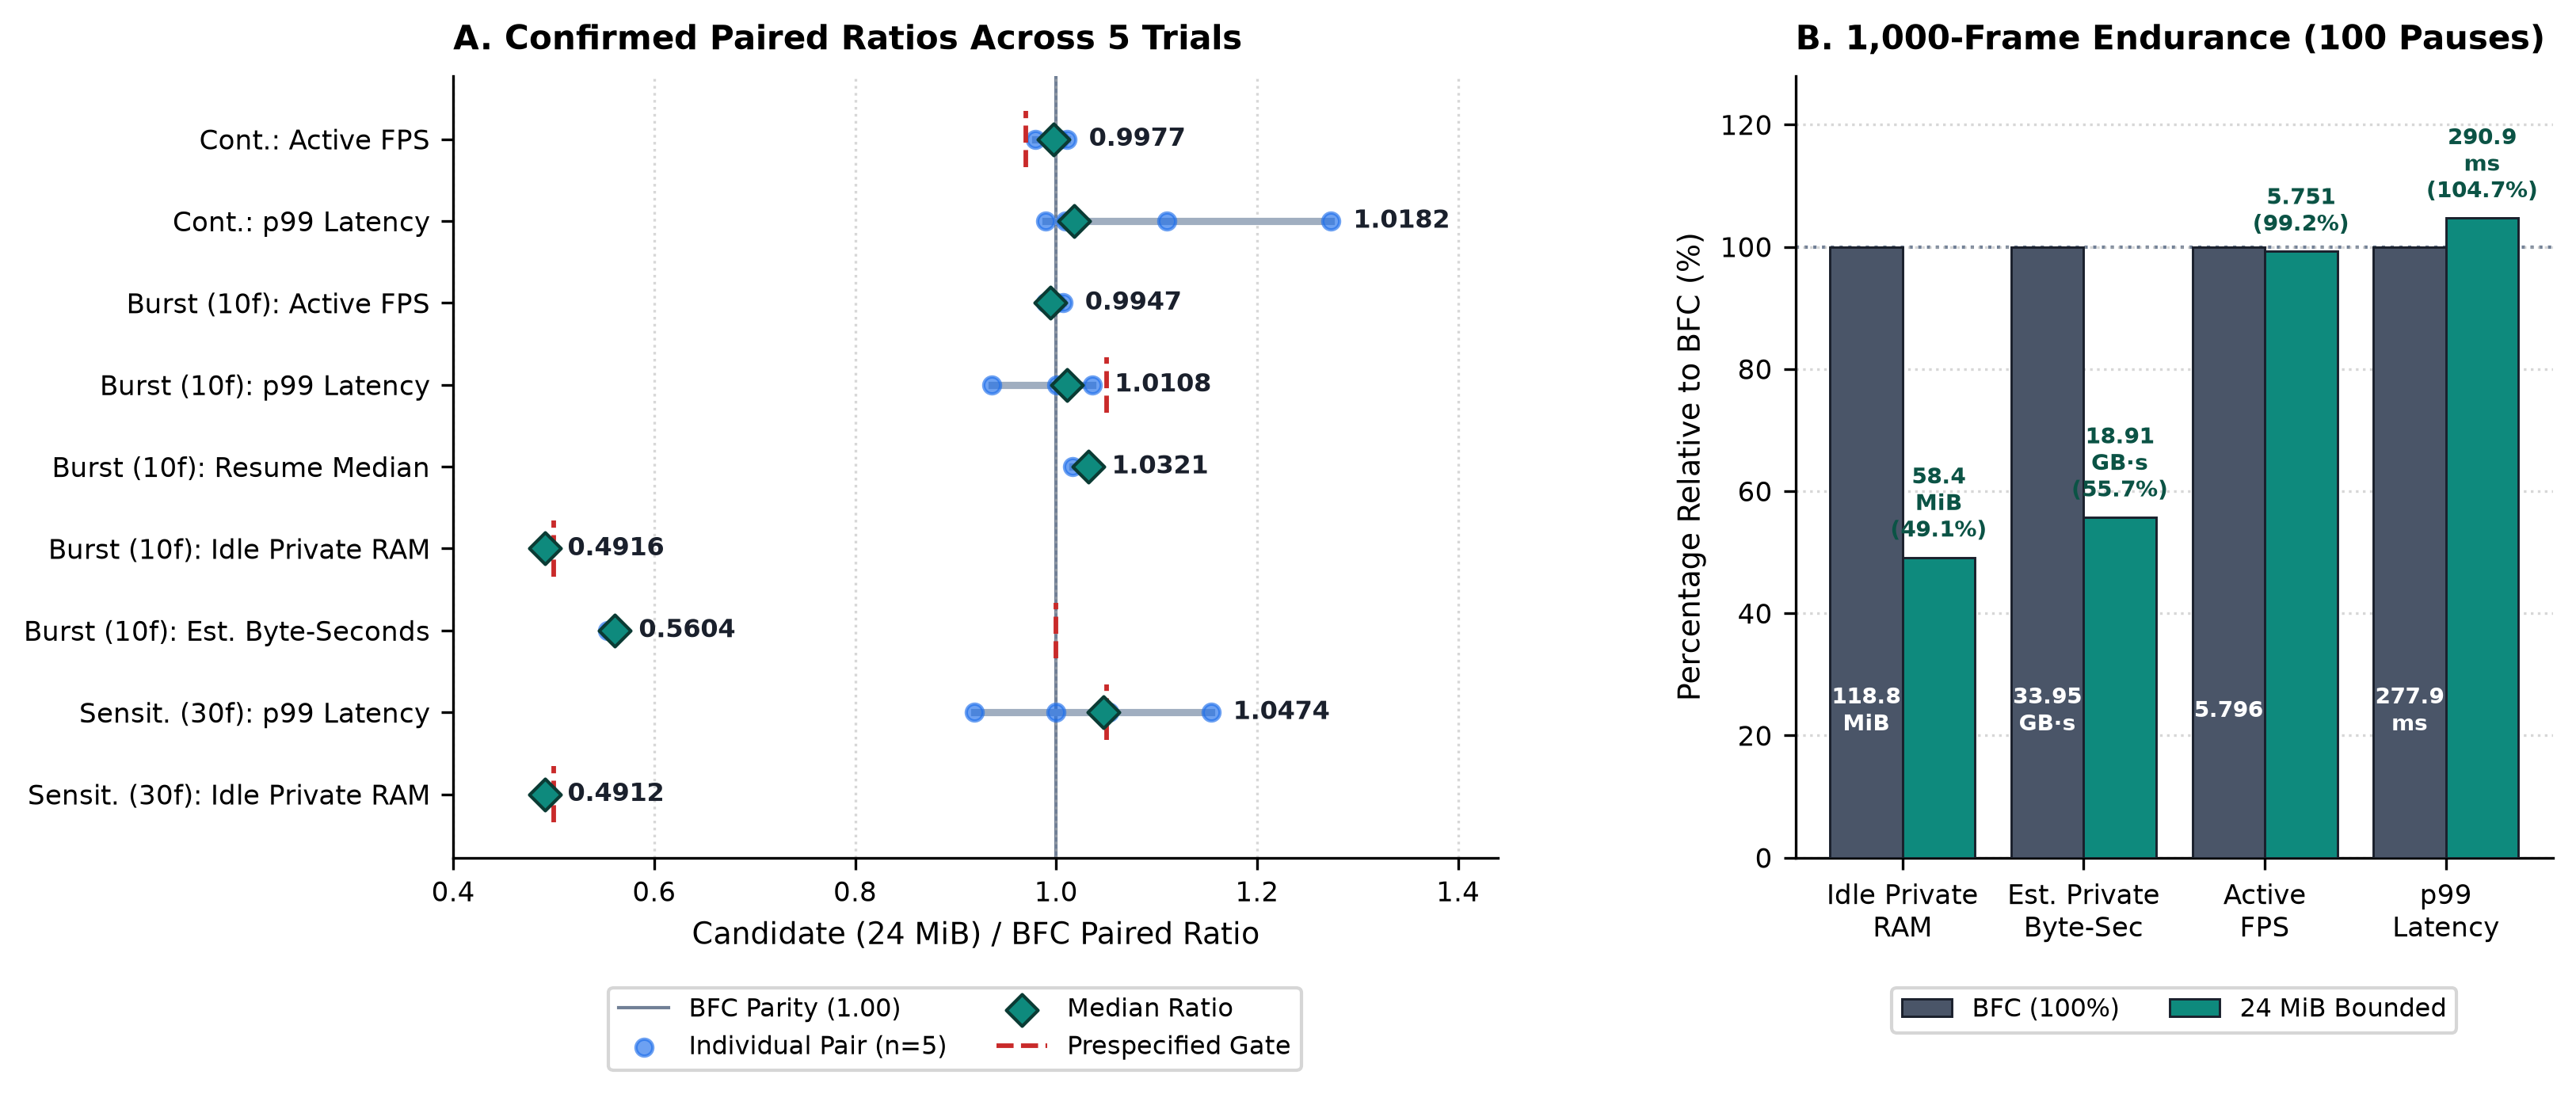
\includegraphics[width=\textwidth]{figures/fig3_confirmation_endurance.png}
  \caption{Confirmed bounded-retention results (\texttt{1fd7ede}). (A) Paired 24~MiB / BFC ratios across five fresh processes per regime showing individual trials, min--max ranges, medians, and pre-registered gates. (B) 1,000-frame endurance comparison across 100 pauses.}
  \label{fig:bounded}
\end{figure*}

\section{Significance, Limitations, and Future Work}
These results demonstrate that dedicated edge vision deployments can recover substantial physical RAM without model compression or numerical approximation. Simply replacing unbounded inference arenas with tuned \texttt{glibc} trimming removes $\sim$40\% of single-stream active peak RSS, while bounded pause reclamation cuts idle private residency in half across quiescent periods without incurring the severe tail-latency penalties of naive zero-retention purging. In multi-camera deployments---where four concurrent sessions retained 390.80~MiB idle private RAM under trimmed BFC versus 88.05~MiB under \texttt{pool\_eager\_trim}---reclaiming idle page bodies directly expands workload co-location headroom on memory-constrained edge gateways. Equally important is our measurement discipline: verifying bit-exact full and caller-retained outputs, querying \texttt{mincore()} inside live sessions, isolating benchmark telemetry from active frame timings, and preserving negative intermediate results (\texttt{c9828c5}) prevent the evaluation blind spots identified in recent allocator literature~\cite{fistanto2026lostbytes,vankempen2026reconsidering}.

Several limitations bound our current findings and define four concrete next steps:
\begin{enumerate}
  \item \textbf{Scheduled Pauses vs.\ Automatic Detection:} Bounded retention currently triggers at explicit harness pause callbacks; integrating an automatic runtime idle detector remains future work.
  \item \textbf{Staggered Multi-Camera Bursts and Real Pressure:} While eager trimming was validated on four live concurrent cameras, bounded pause retention covers a single stream under explicit sleeps. Staggered multi-camera burst schedules and kernel memory-pressure policies driven by measured demand---rather than equating scheduled pauses with system memory pressure---remain to be evaluated.
  \item \textbf{Single-Host and Model Scope:} Results cover a fixed-shape $640 \times 640$ FP32 YOLO26n workload on one Broadwell-DE Xeon D-1548 node with 4~KiB pages. Dynamic input shapes, huge-page settings, and modern ARM or x86 edge microarchitectures require separate validation.
  \item \textbf{Metric Approximation and Dispersion:} \texttt{estimated\_\allowbreak private\_\allowbreak byte\_\allowbreak seconds} samples private residency at frame boundaries and can undercount intra-frame spikes, while the 5\% p99 gate is an assumed research threshold. Individual runs exhibited tail dispersion (continuous p99 max ratio 1.2737; 30-frame max 1.1541), motivating selective page pre-faulting upon burst resumption.
\end{enumerate}

Taken together, the progression from baseline utilization (\texttt{20dc7b8}) through unbudgeted pause purging (\texttt{c9828c5}) to bounded 24~MiB retention (\texttt{1fd7ede}) establishes a practical, reproducible foundation for cutting idle physical DRAM footprints in bursty edge computer vision pipelines without compromising numerical exactness or burst responsiveness.

\bibliographystyle{ACM-Reference-Format}
\bibliography{references}

\end{document}
